

%----------------------------------------------------------------------------------------
%	PACKAGES AND OTHER DOCUMENT CONFIGURATIONS
%----------------------------------------------------------------------------------------

\documentclass[12pt]{article}

\usepackage{polski}
\usepackage[polish]{babel}
\usepackage[utf8]{inputenc} 
\usepackage{datetime}
\usepackage{graphicx}
\usepackage{tikz} 
\usepackage{amsmath}
\usepackage{epstopdf}
\usepackage{multirow}
\usepackage{tabularx}
\usepackage{pdfpages}
%\usepackage[colorlinks=true]{hyperref}
%\usepackage[all]{hypcap}
%\usepackage{showframe} 
\usepackage{geometry}
 \geometry{
 a4paper, 
 left=20mm,
 right=20mm,
 top=20mm,
 bottom=20mm,
 }
 
\renewcommand{\dateseparator}{.}
\newdate{exercise_date}{13}{05}{2014}
\newdate{create_date}{20}{05}{2014}

%----------------------------------------------------------------------------------------

%----------------------------------------------------------------------------------------
% TIKZ PACKAGES
%----------------------------------------------------------------------------------------
 
\usetikzlibrary{arrows, decorations.markings, decorations.pathmorphing, calc,
positioning, intersections, shapes, decorations.pathreplacing}

%----------------------------------------------------------------------------------------

\begin{document}

\begin{titlepage}

\newcommand{\HRule}{\rule{\linewidth}{0.5mm}}
% Defines a new command for the horizontal lines, change thickness here

\center
% Center everything on the page
 
%----------------------------------------------------------------------------------------
%	LOGO SECTION
%----------------------------------------------------------------------------------------


\includegraphics[width=6cm]{../res/img/logo.png}\\[1cm]
% Include a department/university logo - this will require the graphicx package
 
%----------------------------------------------------------------------------------------
 
%----------------------------------------------------------------------------------------
%	HEADING SECTIONS
%----------------------------------------------------------------------------------------

\textsc{\LARGE Akademia Górniczo-Hutnicza \\[0.2cm]
im. Stanisława Staszica w Krakowie}\\[1.5cm]
% Name of your university/college

\textsc{\Large Podstawy Automatyki}\\[0.5cm]
% Major heading such as course name

%----------------------------------------------------------------------------------------
%	TITLE SECTION
%----------------------------------------------------------------------------------------

\HRule \\[0.5cm]
{ \huge \bfseries Dyskretne układy regulacji \\[0.3cm] oraz \\[0.5cm] Analiza
serwomechanizmu \\[0.2cm] przekaźnikowego z wykorzystaniem płaszczyzny
fazowej}\\[0.3cm]
% Title of your document
\HRule \\[1.5cm]
 
%----------------------------------------------------------------------------------------
%	AUTHOR SECTION
%----------------------------------------------------------------------------------------

% \begin{minipage}{0.4\textwidth}
% \begin{flushleft} \large
% \emph{Author:}\\
% Konrad \textsc{Adasiewcz} % Your name
% \end{flushleft}
% \end{minipage}
% ~
% \begin{minipage}{0.4\textwidth}
% \begin{flushright} \large
% \emph{Supervisor:} \\
% dr inż. Paweł \textsc{Rotter} % Supervisor's Name
% \end{flushright}
% \end{minipage}\\[4cm]

% If you don't want a supervisor, uncomment the two lines below and remove the section above
\flushright
\Large \emph{Autorzy:}\\
Konrad \textsc{Adasiewcz}\\[0.1cm] % Your name
Michał \textsc{Maciejewski}\\[3cm] % Your name

%----------------------------------------------------------------------------------------
%	DATE SECTION
%----------------------------------------------------------------------------------------
Data wykonania ćwiczenia: \\
{\large \displaydate{exercise_date}}\\[1cm]


\vfill % Fill the rest of the page with whitespace

\end{titlepage}

\section{Wstęp}

\subsection{Cel ćwiczenia}

Zapoznanie się z charakterystykami skokowymi regulatora: P, PI, PD oraz PID z wyjściem 
ciągłym i dwupołożeniowym oraz zapoznanie się z elementami programowania regulatora 
EFTRONIK X.

\subsection{Opis stanowiska} 

Stanowisko ma postać szafy z wbudowanym w górnej części regulatorem, wskaźnikami
poziomu sygnałów: wejściowego i wyjściowego z regulatora oraz wskaźnikami stanu wejść/wyjść 
binarnych i przełącznikami służącymi do zadania sygnału \textit{1} lub
\textit{0} na wejścia binarne. Poniżej wskaźników znajdują się gniazda do
pomiaru sygnału wejściowego oraz sygnału wyjściowego. Ponadto w górnej części płyty czołowej
znajduje się włącznik sieciowy oraz poniżej regulatora przełączniki: P1
regulator/układ regulacji czarny oraz wyjście ciągłe/dwupołożeniowe P2
niebieski – wyjście ciągłe, czerwony – wyjście dwupołożeniowe.
Poniżej regulatora znajduje się szuflada zawierająca źródła prądowe 0 – 5 [mA]: stacyjki ADS-
31 oraz zadajnik stałowartościowy ANS-11.

\begin{figure}[!htb]
	\begin{center}
		\includegraphics[page=19,width=17cm,trim=2.5cm 4.8cm 3cm 17cm,clip]
		{../res/img/schemat_stanowiska.pdf}
	\end{center}
	\caption{Schemat stanowiska}
\end{figure}

\subsection{Algorytm regulacyjny}

Algorytm regulacji PID wg. DTR regulatora EFTRONIK X jest opisany transmitancją:

\begin{equation}
	G(s)=k\left(1+\frac{1}{T_is}+\frac{T_ds}{T_d\alpha s+1}\right)
\end{equation}

gdzie $\alpha=0.125$.

\newpage

\section{Przebieg ćwiczenia}

Podczas ćwiczenia ściągnęliśmy szereg odpowiedzi regulatora na skok jednostkowy
dla różnych jego nastaw, wyjścia ciągłego oraz PWM.

\subsection{Wyjście ciągłe}

\begin{figure}[!htb]
	\begin{center}
		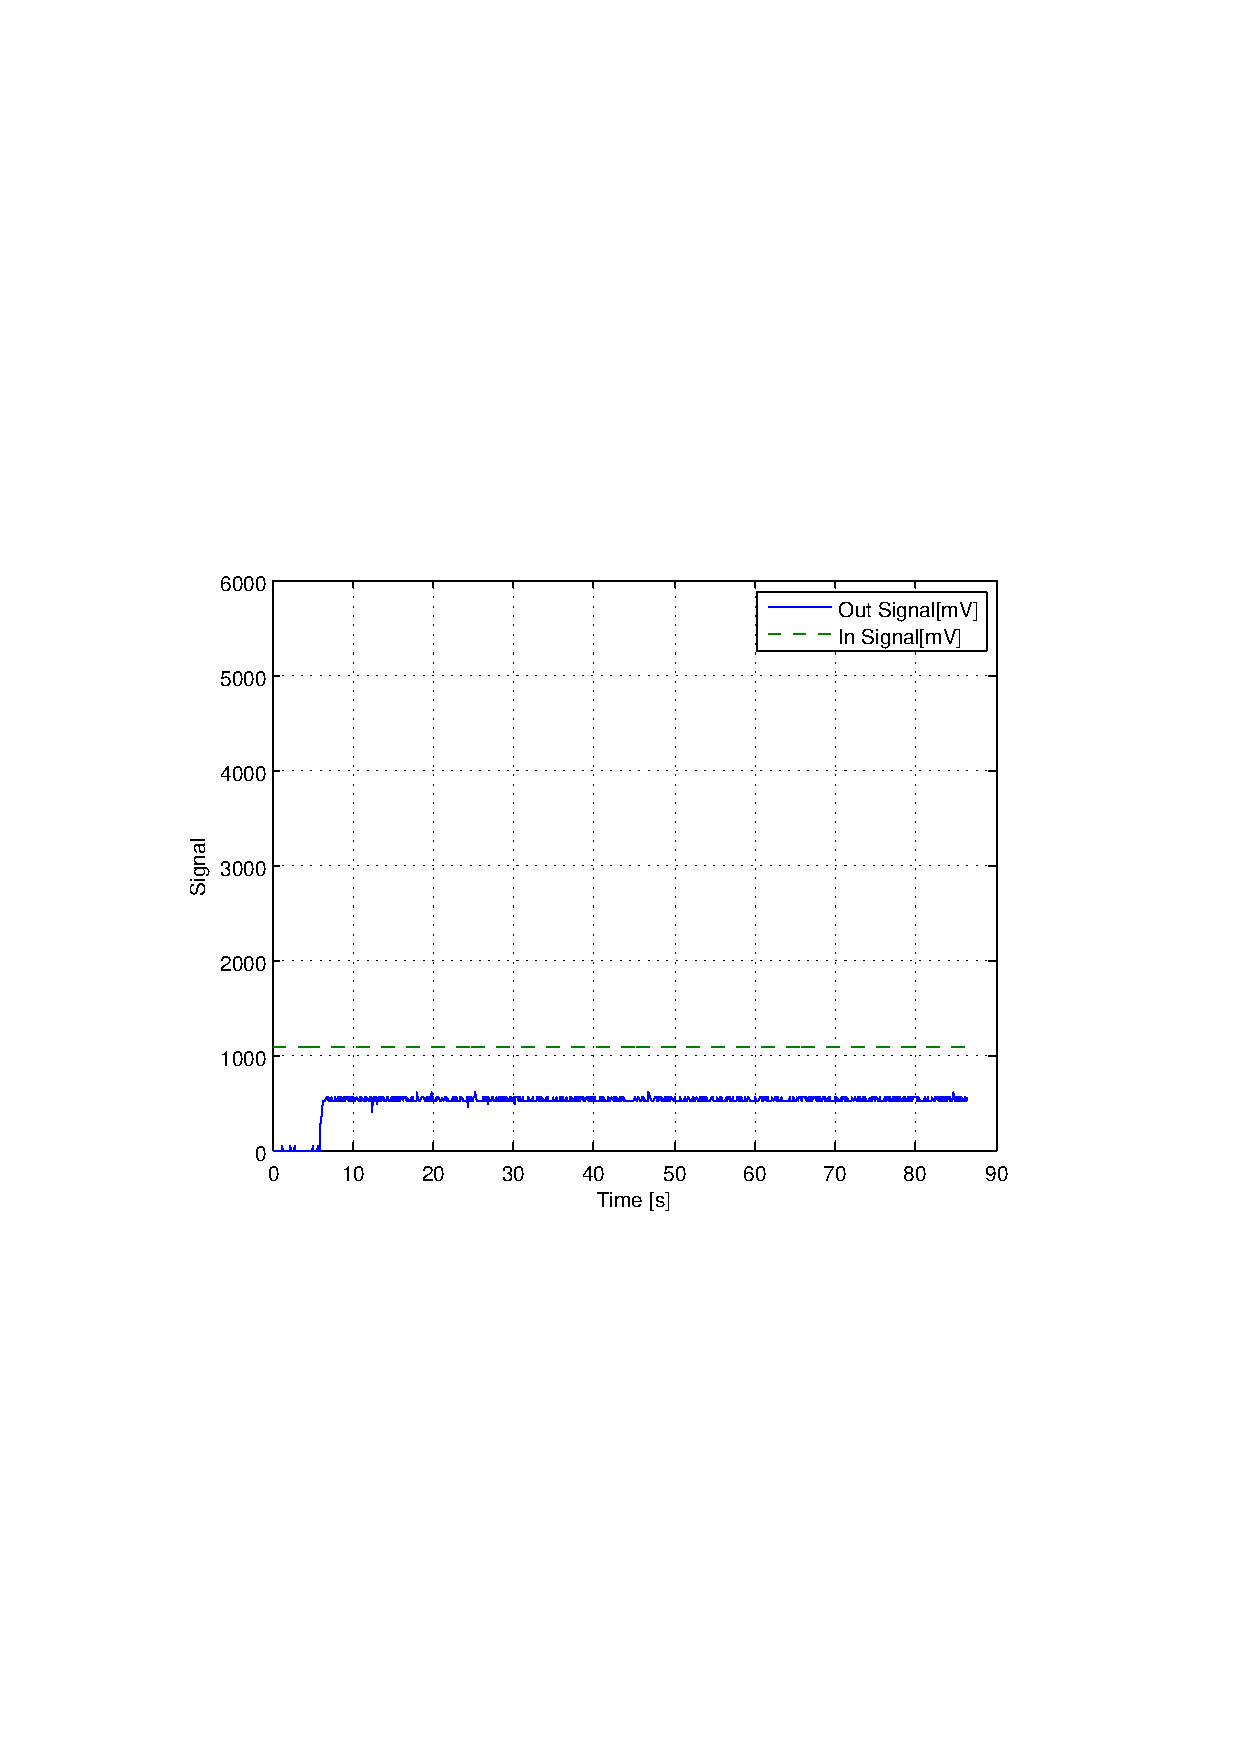
\includegraphics[width=15cm,trim=3cm 9cm 3cm 9cm,clip]
		{../res/img/cont_0,5_0_0.pdf}
	\end{center}
	\caption{Odpowiedź regulatora dla nastaw $k=0.5[-]$, $T_i$ off, $T_d$ off}
\end{figure}

Podawany skok jest powtarzany na wyjściu regulatora, ma jednak wartość zmienioną
proporcjonalnie do współczynnika $k$.

\newpage

\begin{figure}[!htb]
	\begin{center}
		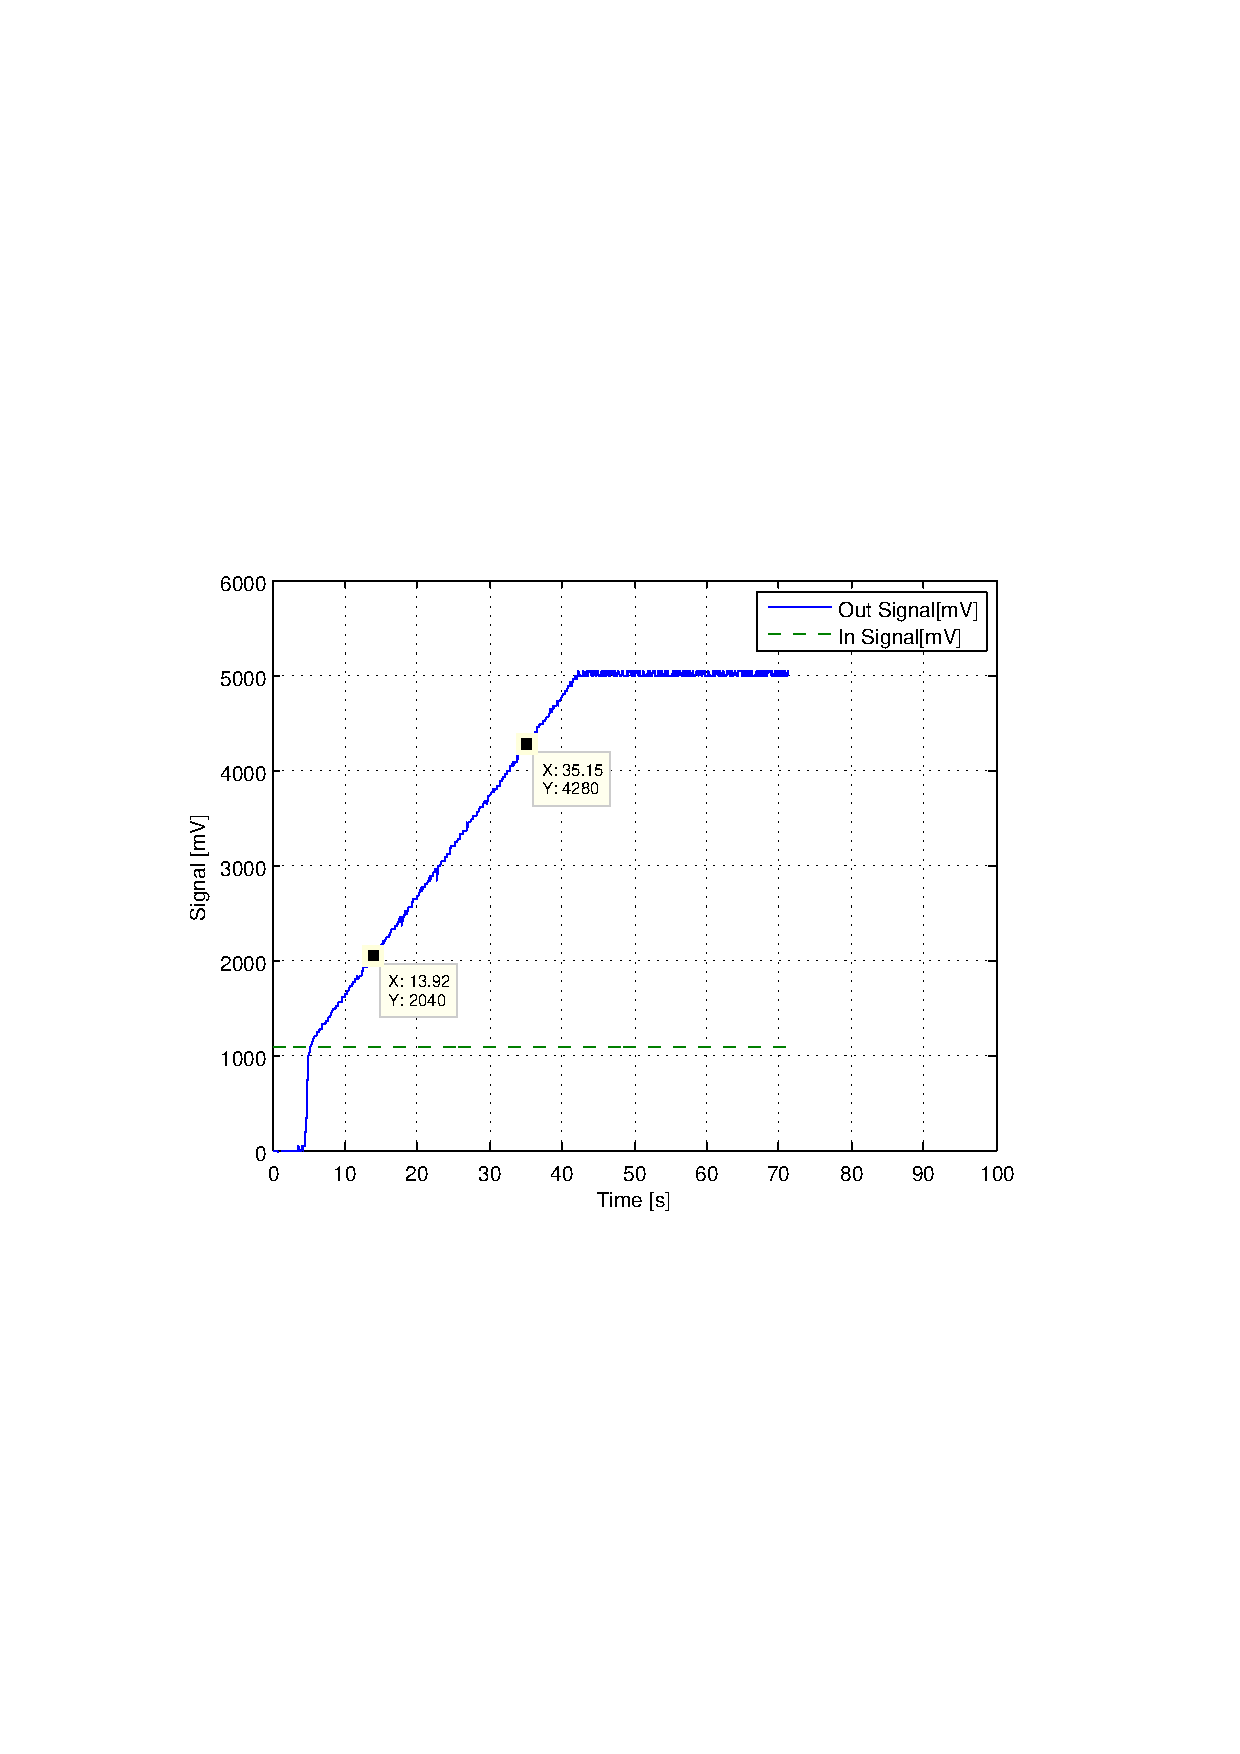
\includegraphics[width=15cm,trim=3cm 9cm 3cm 9cm,clip]
		{../res/img/cont_1_10_0.pdf}
	\end{center}
	\caption{Odpowiedź regulatora dla nastaw $k=1[-]$, $T_i=10[s]$, $T_d$ off}
\end{figure}

Odpowiedź regulatora PI. Parametr $k$ możemy odczytać dzieląc wartość napięcia
wyjściowego na regulatorze w chwili tuż po zadaniu skoku, przez wartość skoku
wymuszającego. Stosunek $\frac{k}{T_i}$ odczytać można wyznaczając współczynnik
nachylenia prostej narastającej odpowiedzi. $\frac{k}{T_i}=\frac{\Delta
y}{\Delta t}=0,106$

\newpage

\begin{figure}[!htb]
	\begin{center}
		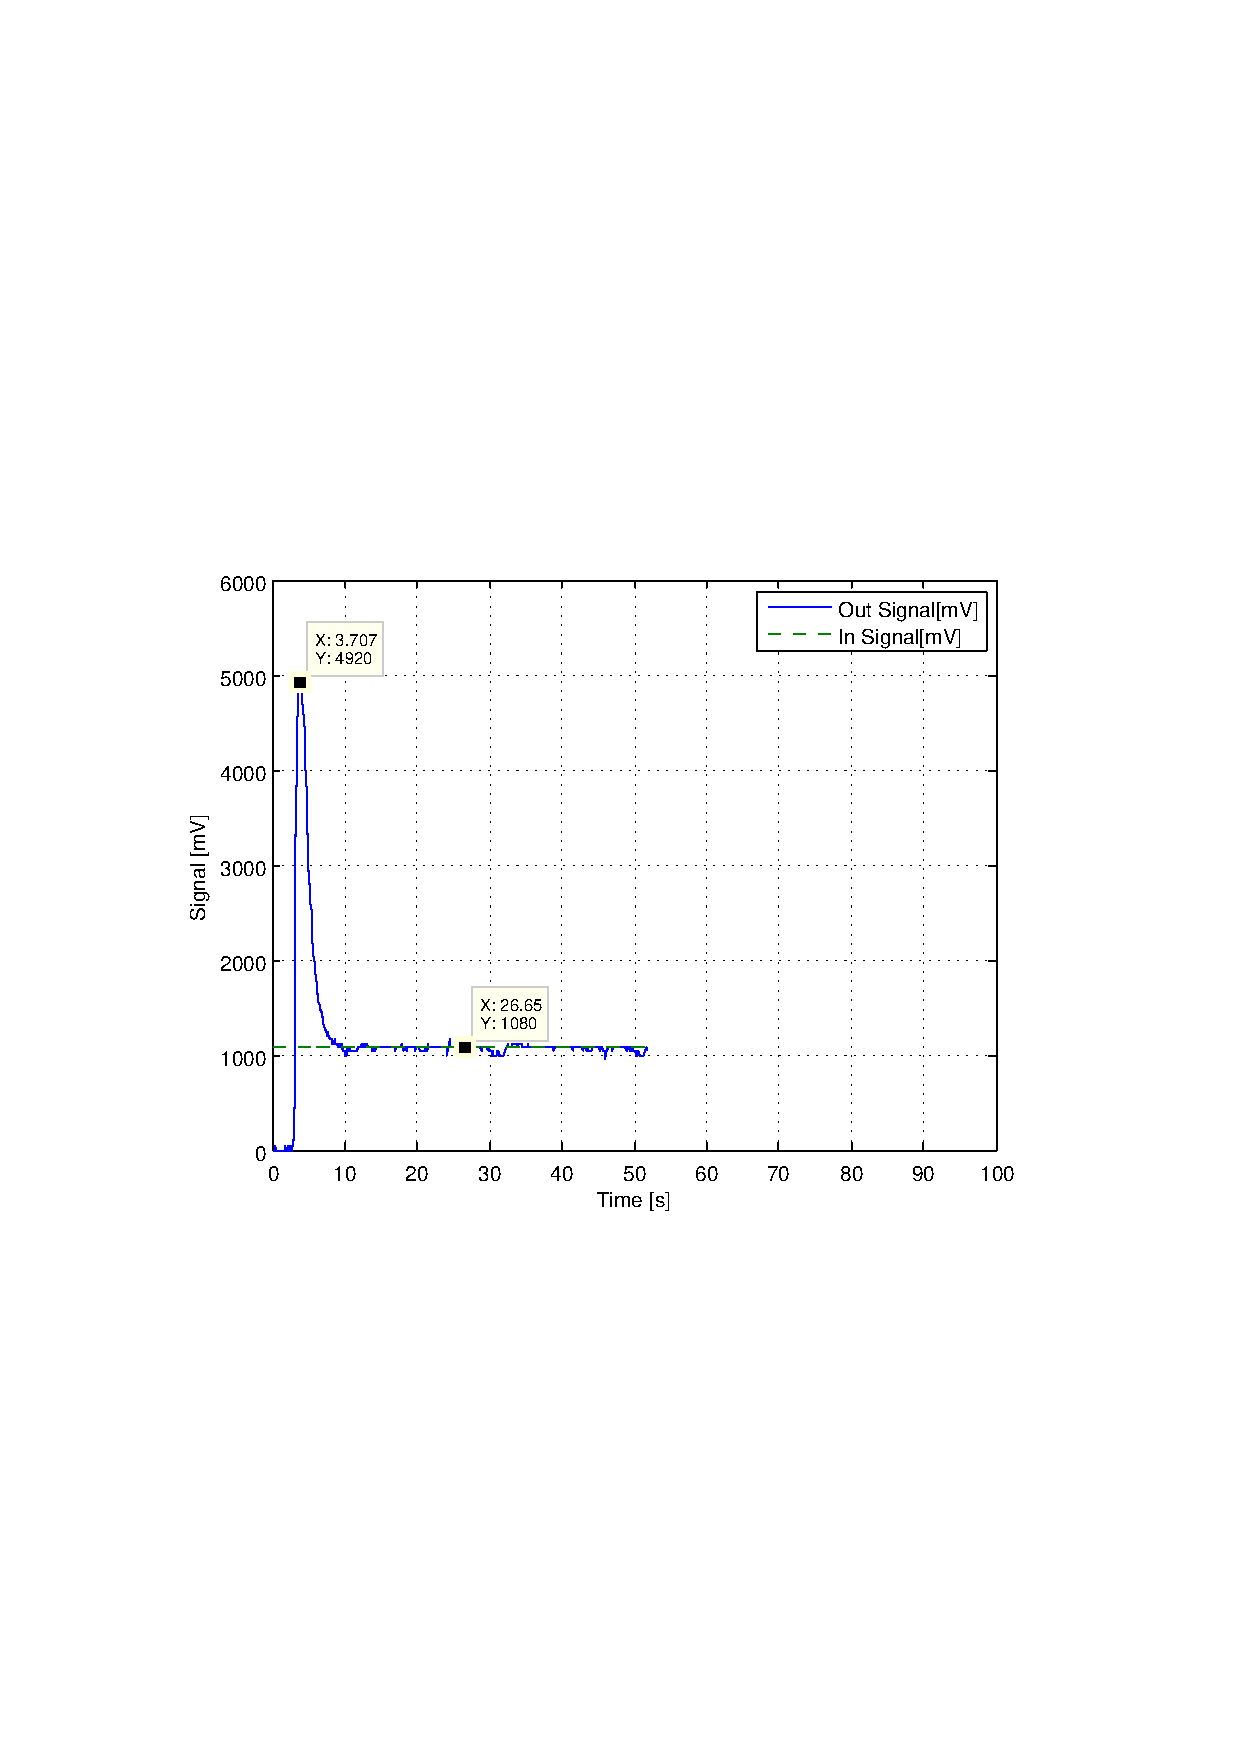
\includegraphics[width=15cm,trim=3cm 9cm 3cm 9cm,clip]
		{../res/img/cont_1_0_10.pdf}
	\end{center} 
	\caption{Odpowiedź regulatora dla nastaw $k=1[-]$, $T_i$ off, $T_d=10[s]$}
\end{figure}

Odpowiedź regulatora PD. Parametry członu różniczkującego są dużo trudniejsze do
wyznaczenia z odpowiedzi skokowej regulatora niż parametry $k$ oraz $T_i$,
ponieważ przeszkodą jest dodatkowy parametr inercji członu różniczkującego, oraz
ograniczone możliwości napięciowe wyjścia regulatora. Transmitancja regulatora
ma taką postać, że wyznaczenie parametrów członu różniczkującego jest
niemożliwe, ponieważ szpilka w momencie podania skoku na regulator powinna mieć
amplitudę niezależną od parametru $T_d$ i powinna wynosić
$k(1+\frac{1}{\alpha})=9k$.

\newpage

\begin{figure}[!htb]
	\begin{center}
		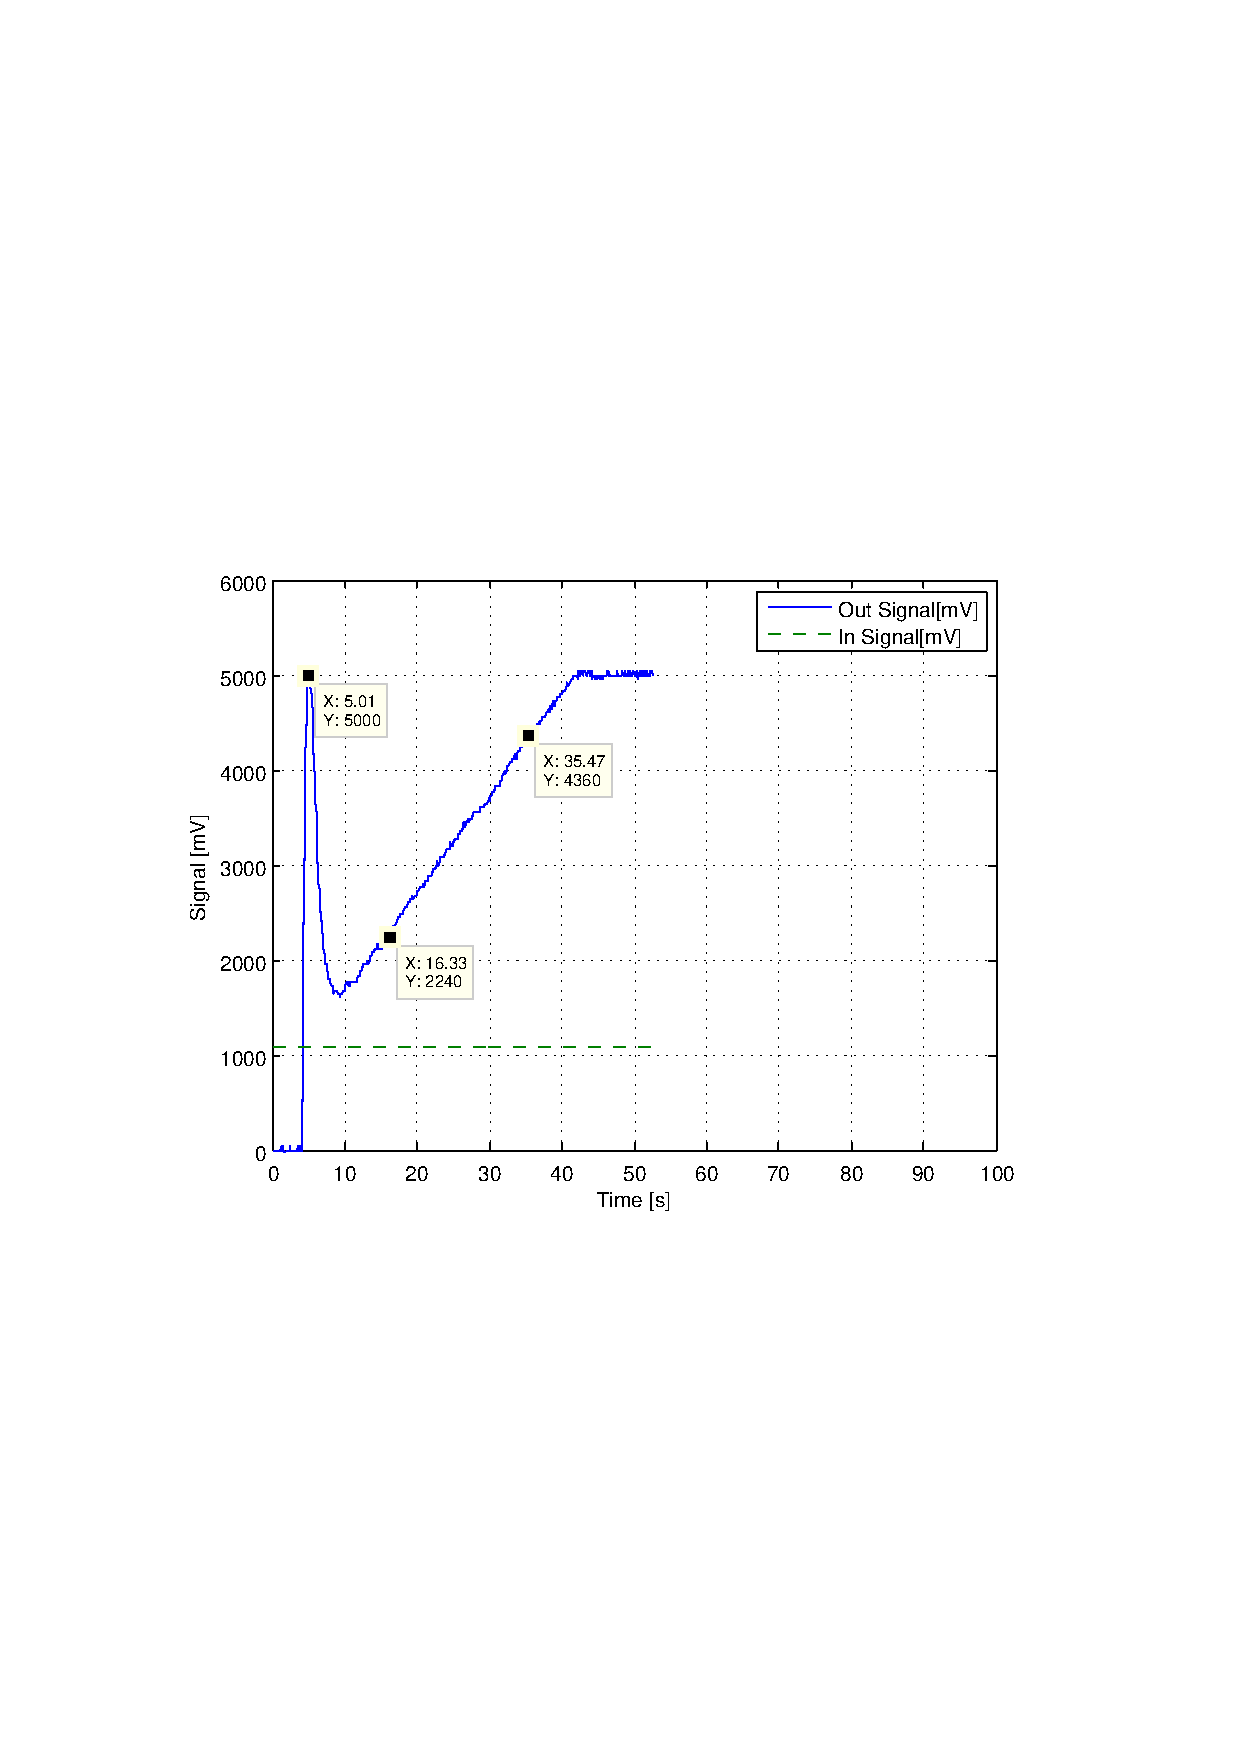
\includegraphics[width=12cm,trim=3cm 9cm 3cm 9cm,clip]
		{../res/img/cont_1_10_10.pdf}
	\end{center}
	\caption{Odpowiedź regulatora dla nastaw $k=1[-]$, $T_i=10[s]$, $T_d=10[s]$}
\end{figure}

\begin{figure}[!htb]
	\begin{center}
		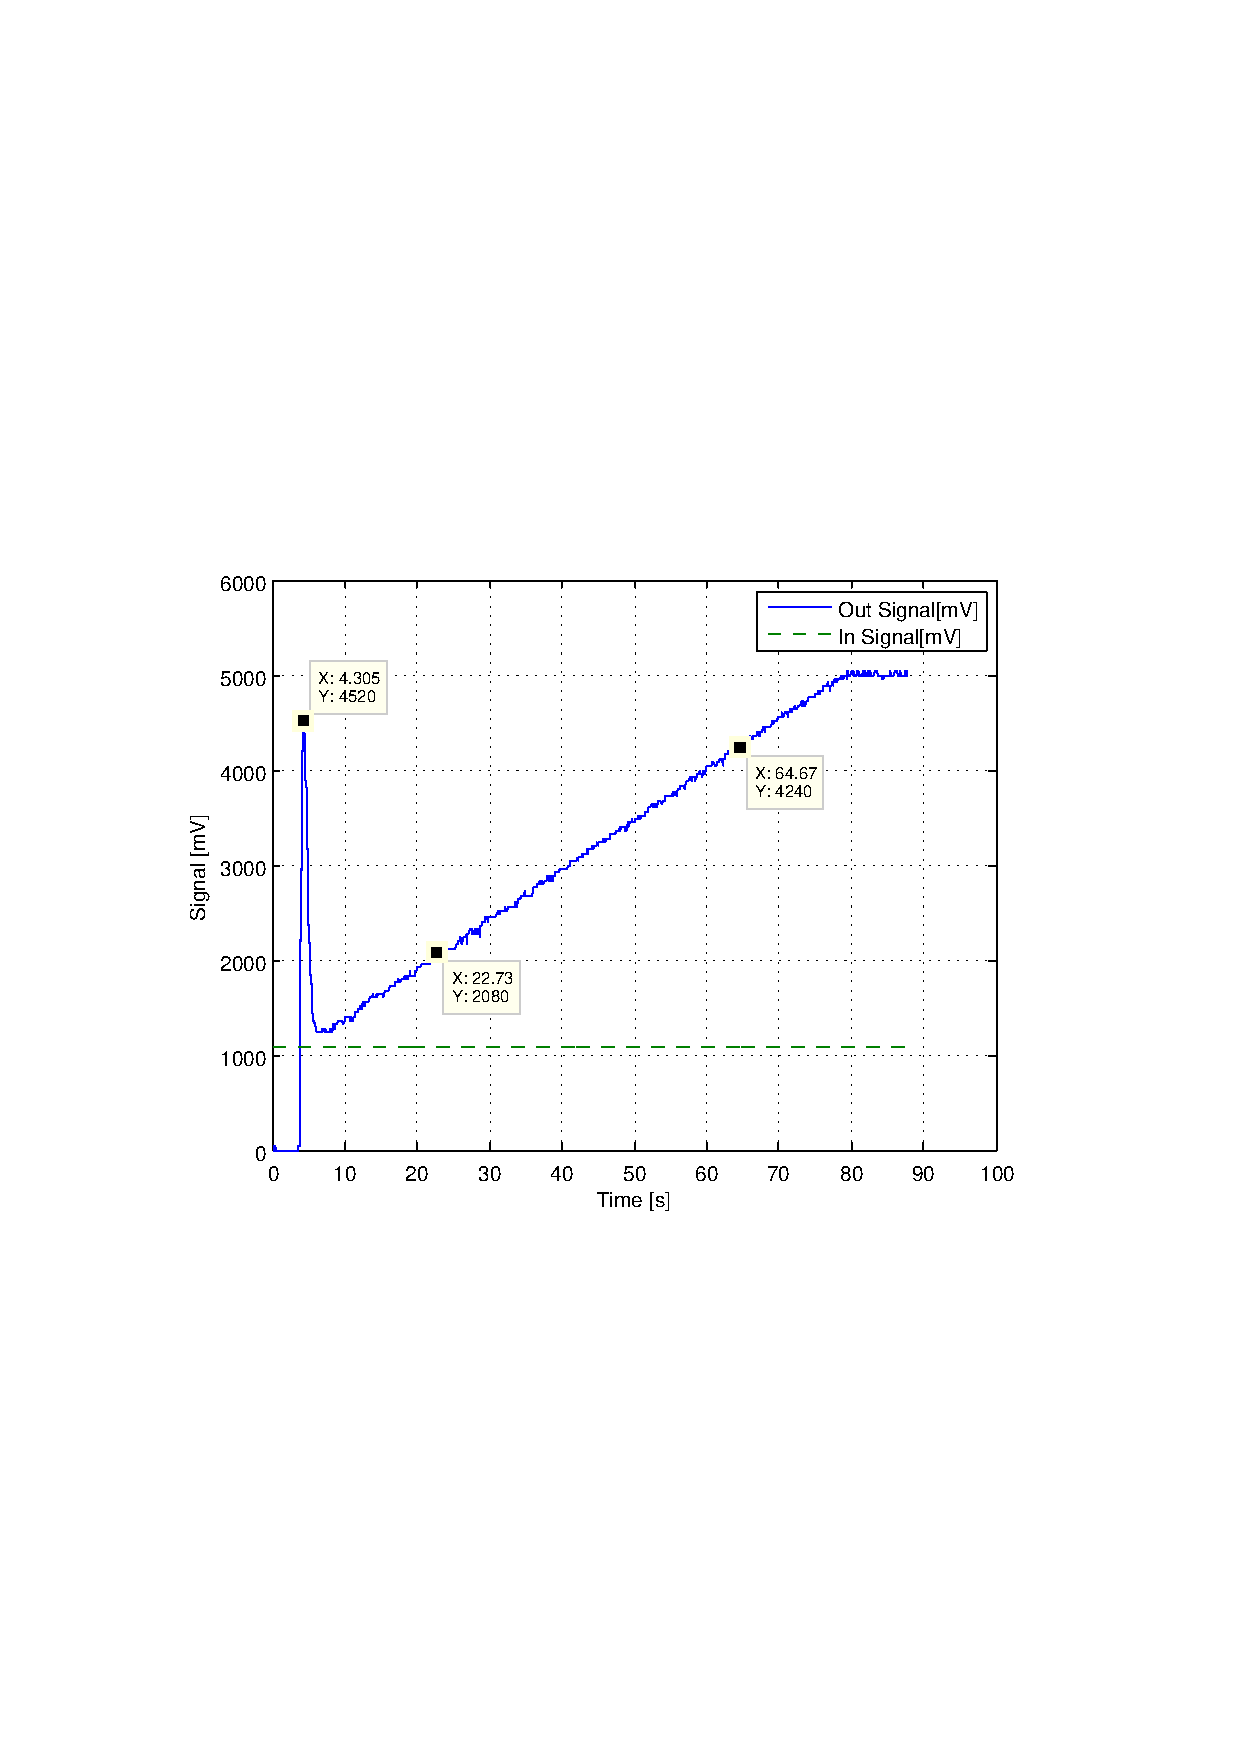
\includegraphics[width=12cm,trim=3cm 9cm 3cm 9cm,clip]
		{../res/img/cont_1_20_5.pdf}
	\end{center} 
	\caption{Odpowiedź regulatora dla nastaw $k=1[-]$, $T_i=20[s]$,
	$T_d=5[s]$}
\end{figure}

Z odpowiedzi pełnych regulatorów można odczytać jedynie parametr
$\frac{k}{T_i}$, ponieważ wszystkie inne parametry prykryte są oddziaływaniem
części różniczkującej regulatora.

\newpage

\subsection{Wyjście PWM}

\begin{figure}[!htb]
	\begin{center}
		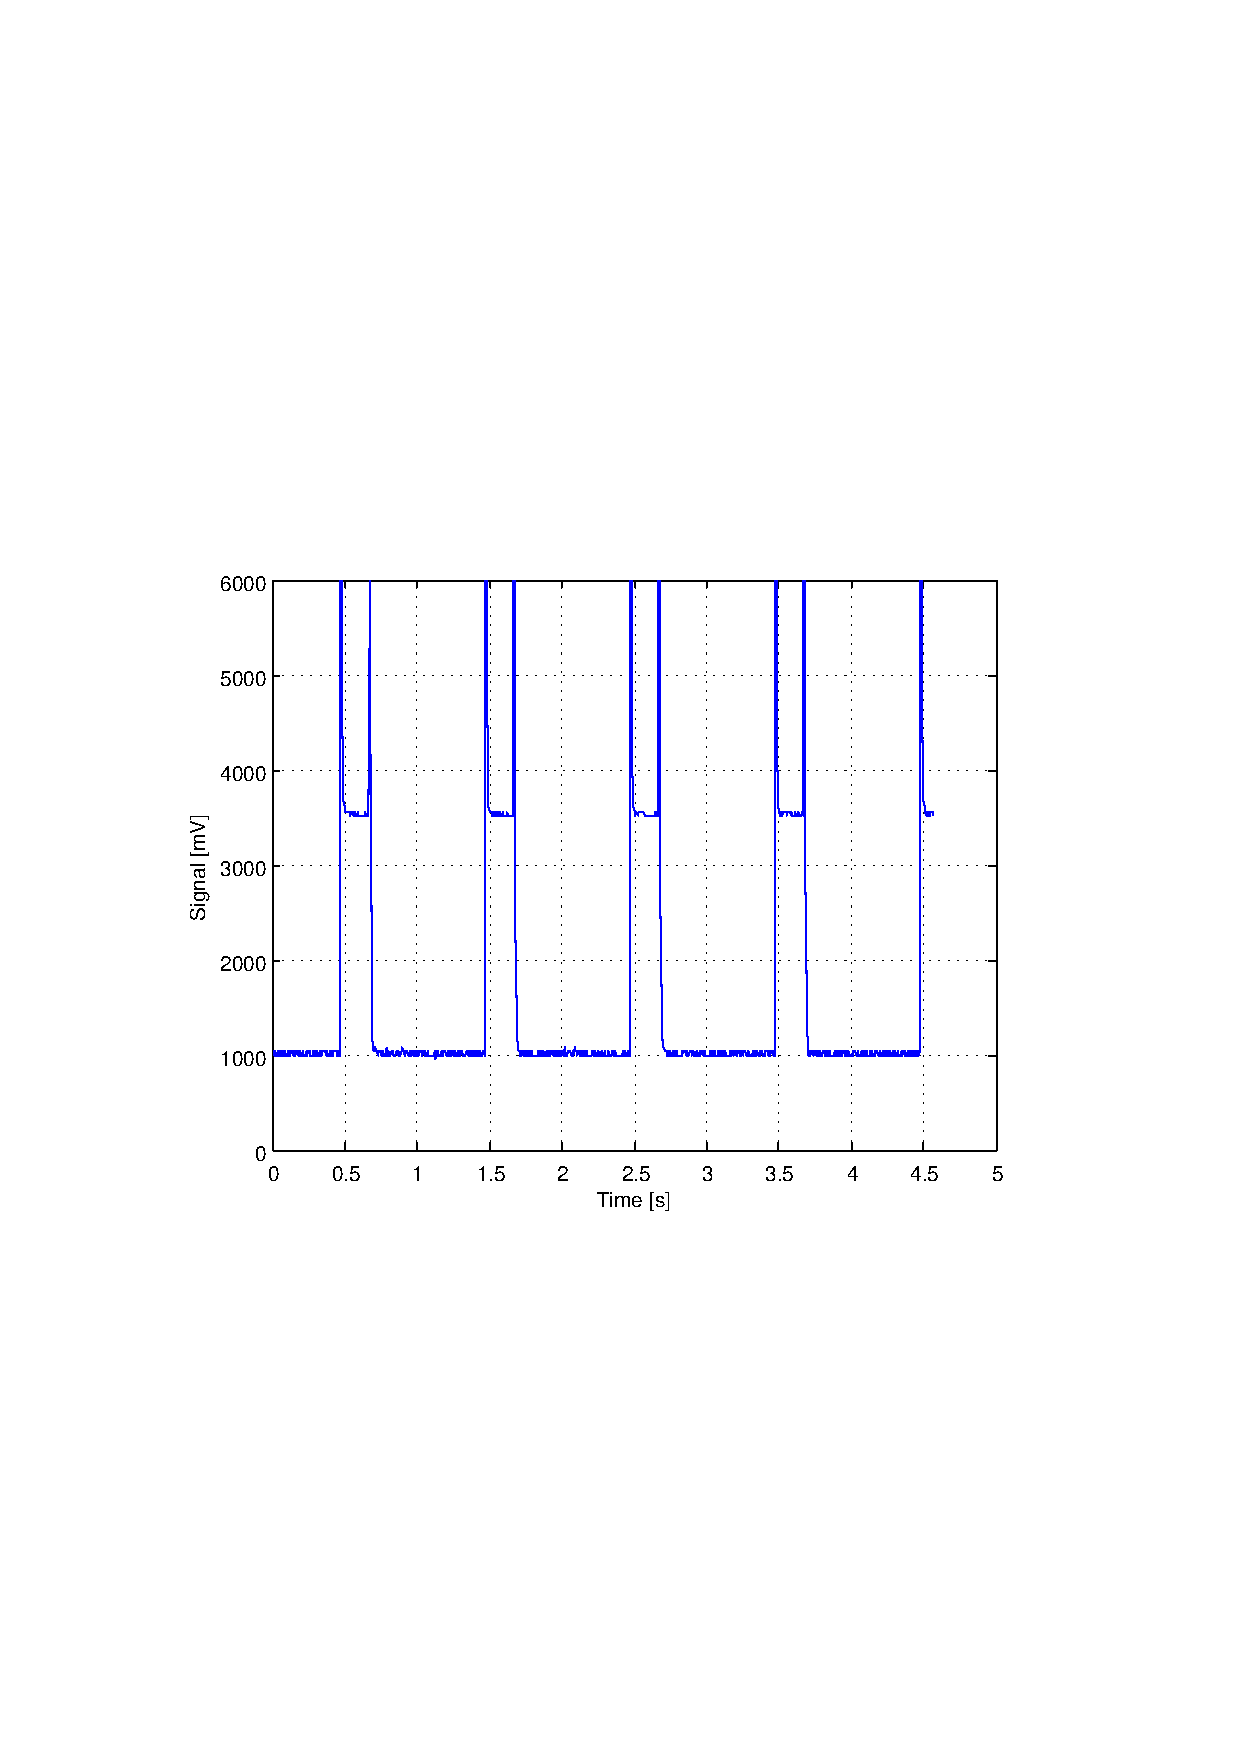
\includegraphics[width=15cm,trim=3cm 9cm 3cm 9cm,clip]
		{../res/img/dism_20_1.pdf}
	\end{center} 
	\caption{Odpowiedź regulatora w trybie dwupołożeniowym o okresie impulsowania
	$1[s]$ i wartości $20\%$ wartości maksymalnej}
\end{figure}

W trybie pracy PWM sygnałem wyjściowym regulatora nie jest wartość napięcia
wyjściowego, lecz stosunek czasu trwania wysokiego stanu wyjścia do sumy czasów
stanu wysokiego i niskiego. W ten sposób regulujemy średnią wartością energii
dostarczanej do obiektu, jednocześnie oszczędzając na stratach związanych z
ograniczaniem sygnału regulatora(wzmacniacz analogowy).

\newpage

\begin{figure}[!htb]
	\begin{center}
		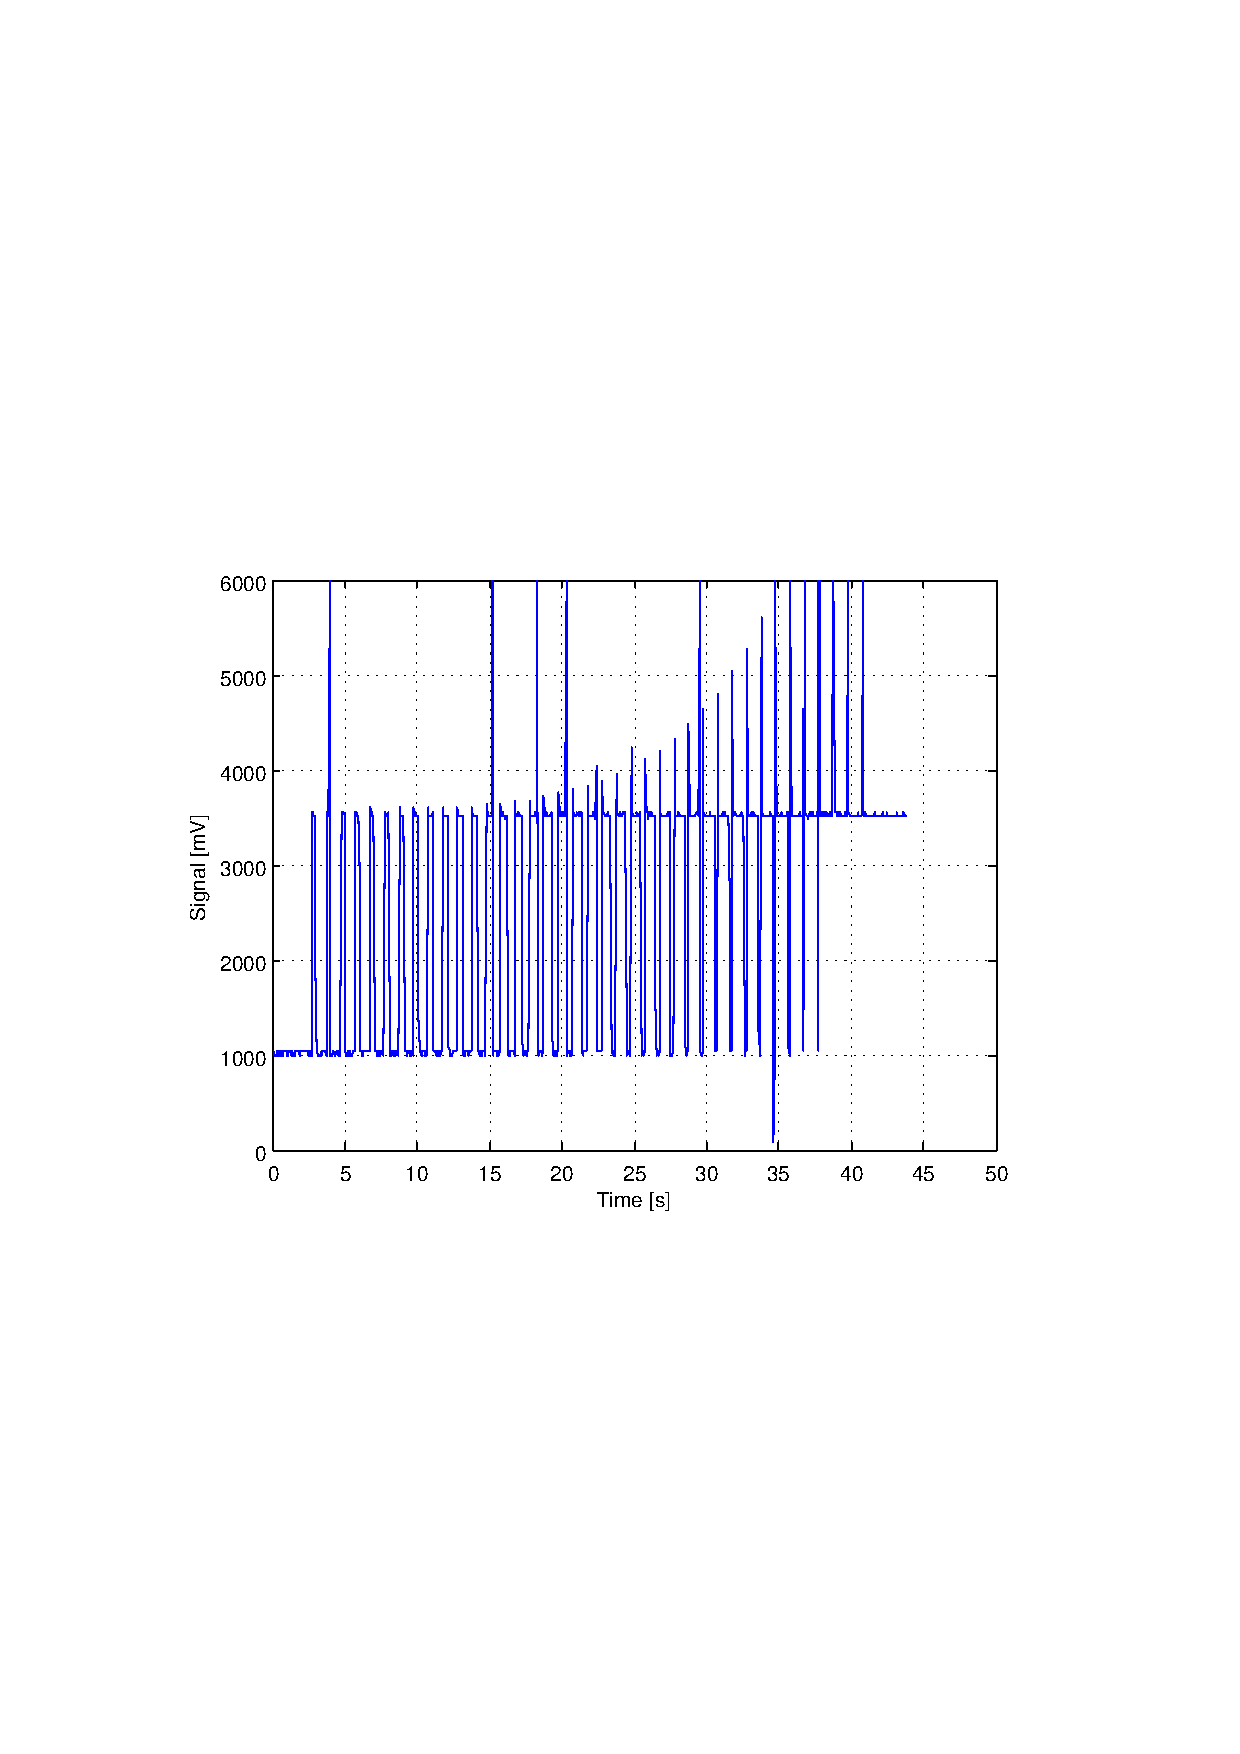
\includegraphics[width=12cm,trim=3cm 9cm 3cm 9cm,clip]
		{../res/img/dis_1_10_0.pdf}
	\end{center} 
	\caption{Odpowiedź regulatora w trybie dwupołożeniowym o okresie impulsowania
	$1[s]$ i nastawach $k=1[-]$, $T_i=10[s]$, $T_d$ off}
\end{figure}

Jak widać regulator zachowuje się jak powinien, odpowiadając na skok wartością
proporcjonalną do niego i liniowo rosnąc aż do nasycenia.

\begin{figure}[!htb]
	\begin{center}
		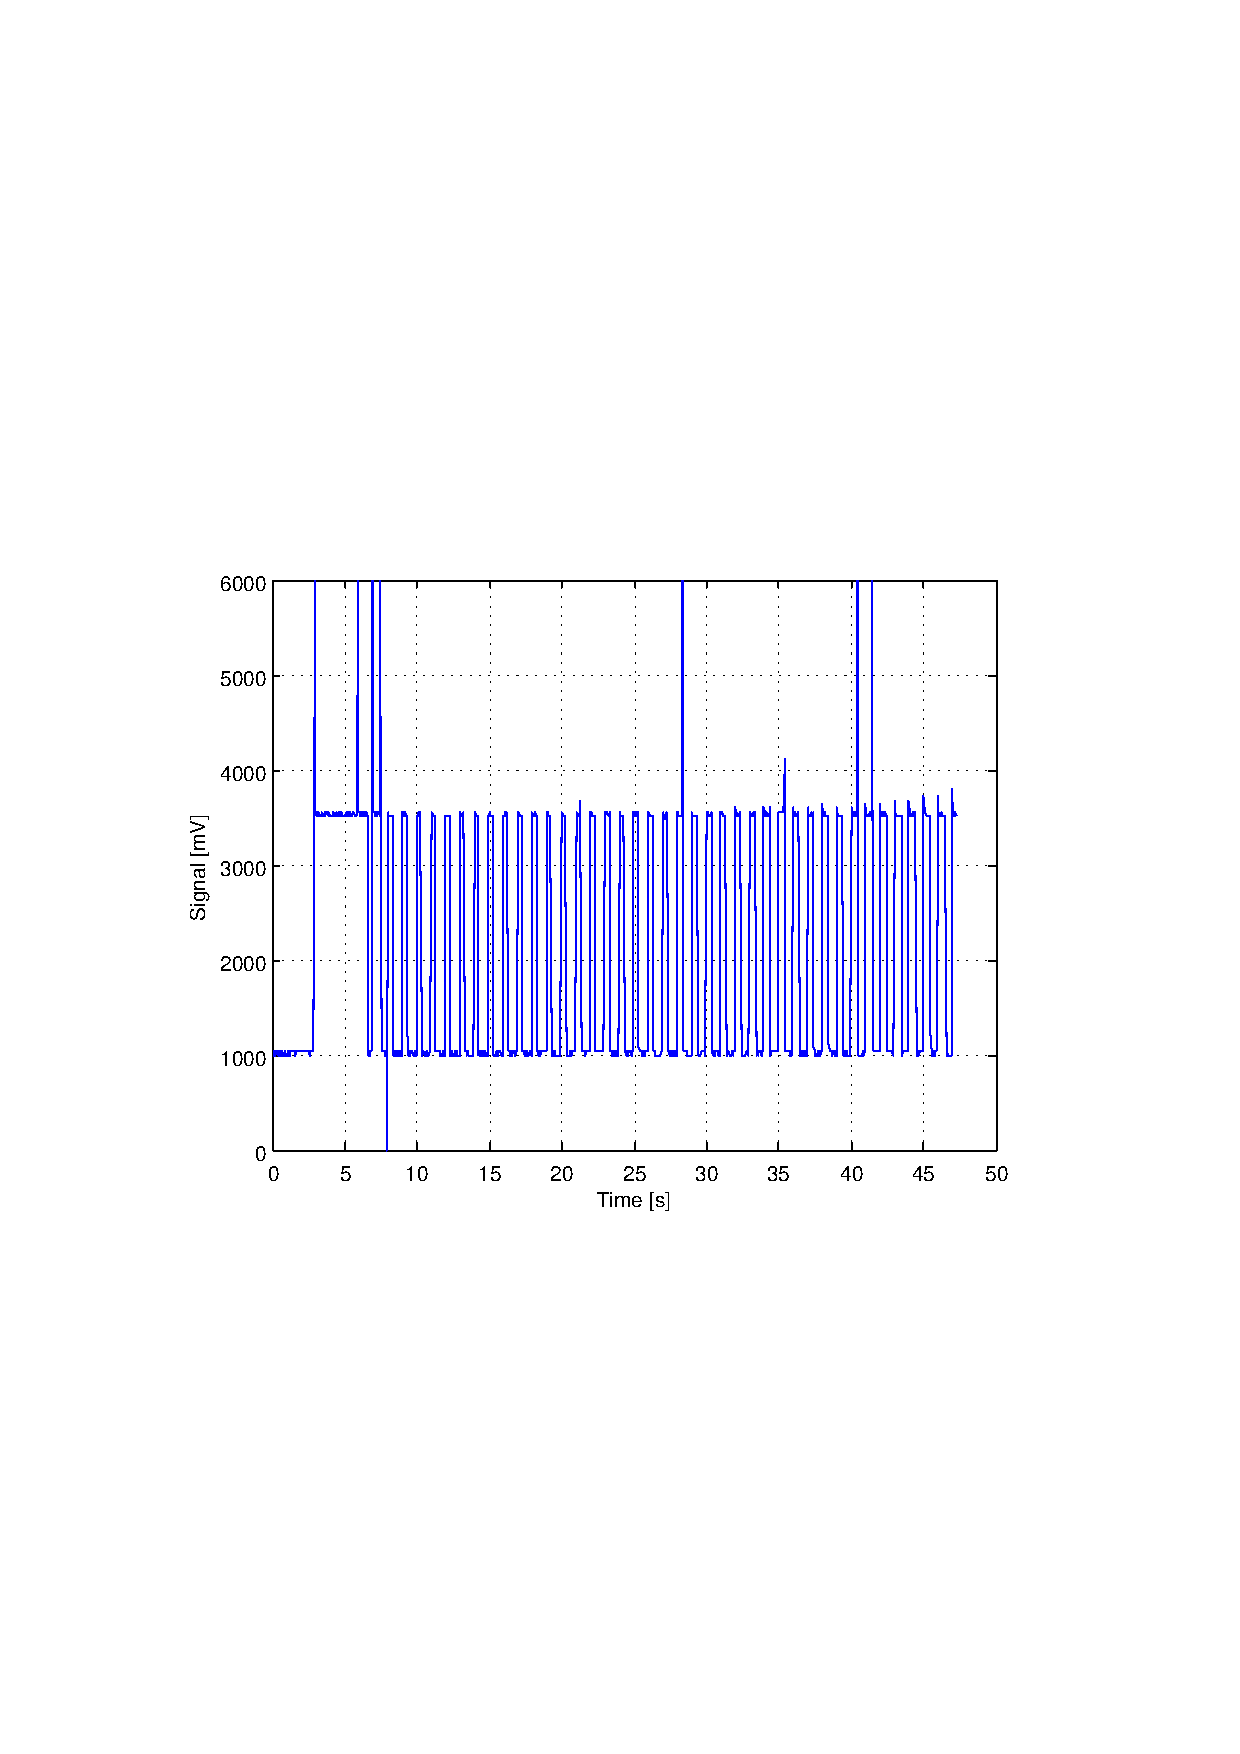
\includegraphics[width=12cm,trim=3cm 9cm 3cm 9cm,clip]
		{../res/img/dis_1_0_10.pdf}
	\end{center} 
	\caption{Odpowiedź regulatora w trybie dwupołożeniowym o okresie impulsowania
	$1[s]$ i nastawach $k=1[-]$, $T_i$ off, $T_d=10[s]$}
\end{figure}

Również w przypadku regulatora PD zachowuje się tak jak regulator w przypadku
wyjścia ciągłego, jednak ze zmienioną postacią sygnału wyjściowego.

\newpage

\begin{figure}[!htb]
	\begin{center}
		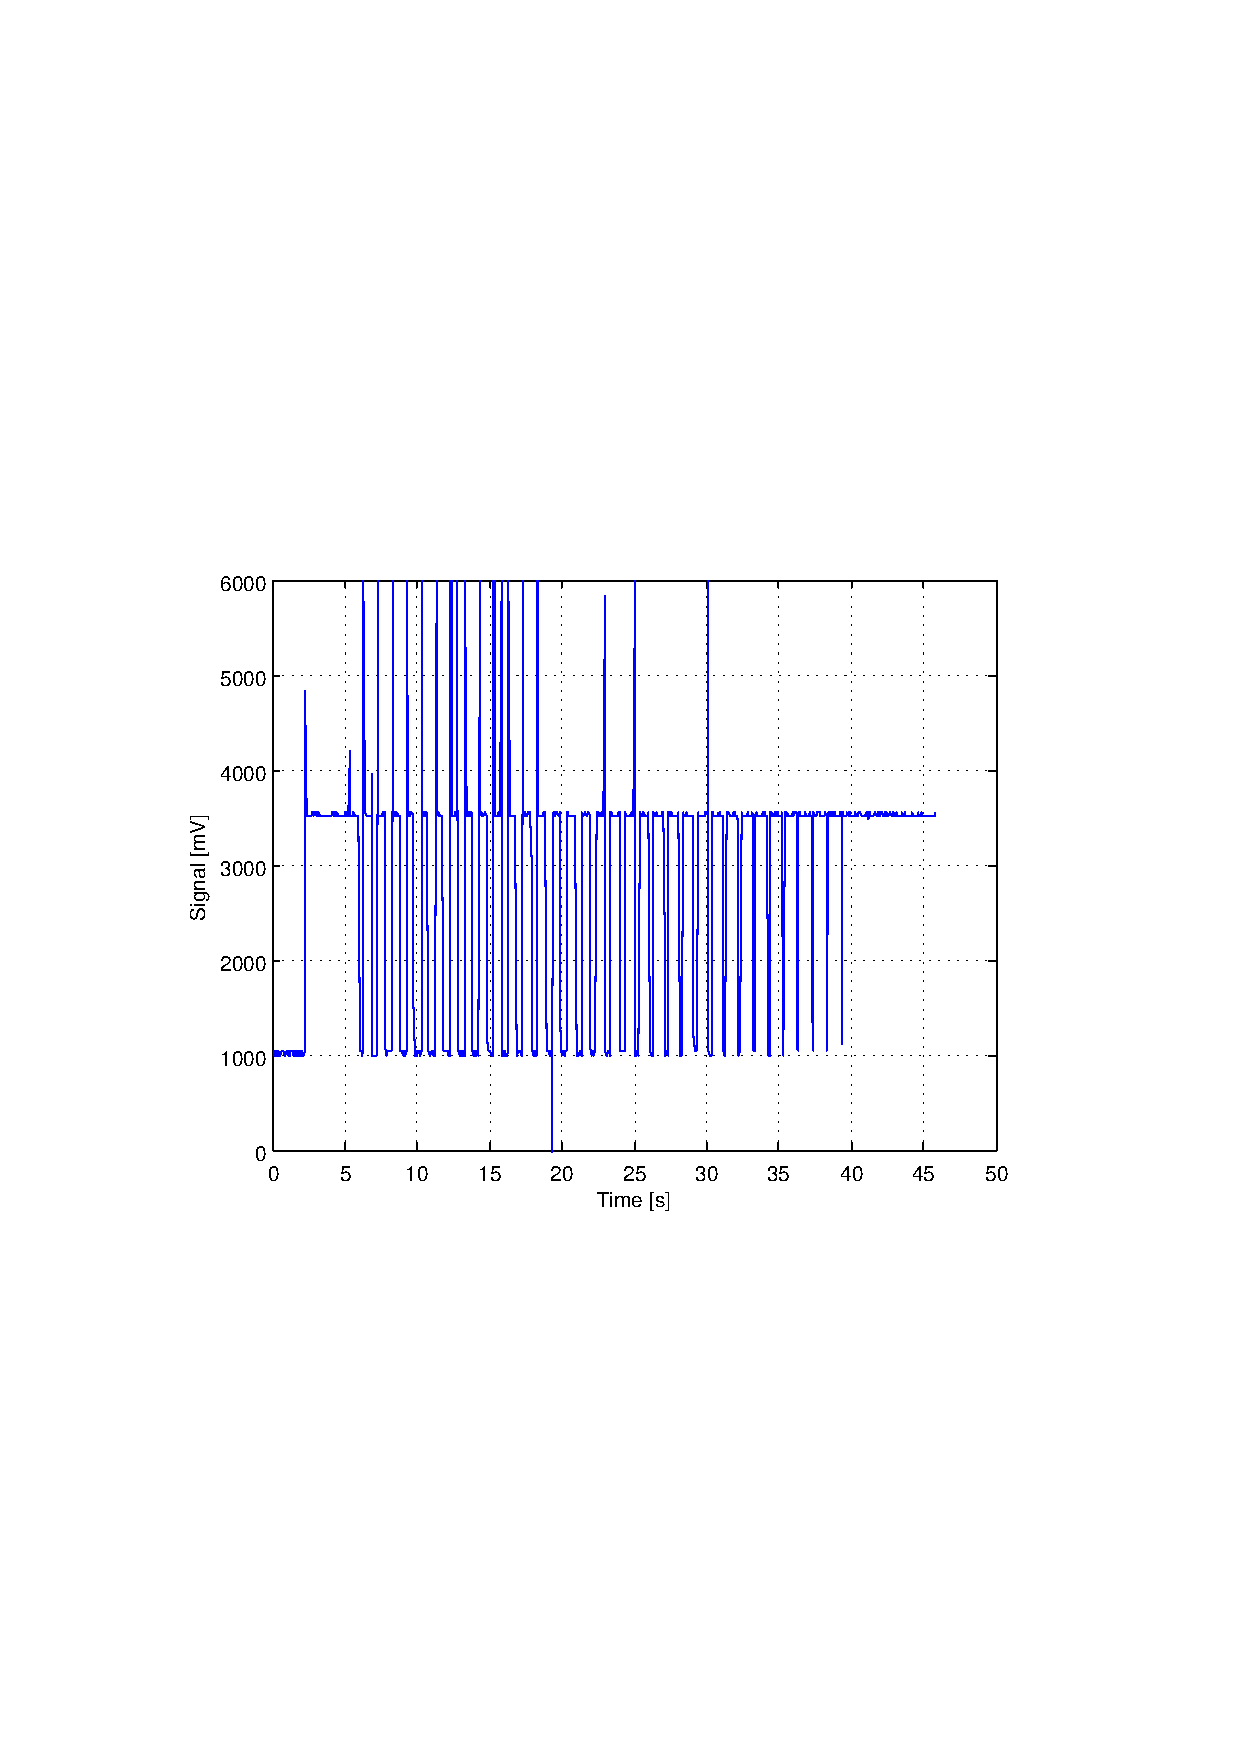
\includegraphics[width=12cm,trim=3cm 9cm 3cm 9cm,clip]
		{../res/img/dis_1_10_20.pdf}
	\end{center} 
	\caption{Odpowiedź regulatora w trybie dwupołożeniowym o okresie impulsowania
	$1[s]$ i nastawach $k=1[-]$, $T_i=10$, $T_d=20[s]$}
\end{figure}

Jak w przypadku regulatora z wyjściem ciągłym dużą trudność sprawia odczytanie
jego parametrów, dodatkowym utrudnieniem jest tutaj nieoczywista wartość sygnału
wyjściowego, którą należy wyliczyć porównując chwilowe czasy stanów wysokich i
niskich sygnału napięciowego regulatora.

\section{Wnioski i spostrzeżenia}

Ćwiczenie przebiegło prawidłowo, wszystkie zarejestrowane odpowiedzi odpowiadają
oczekiwaniom, a możliwe do odczytania parametry zgadzają się z tymi zadanymi w
regulatorze.

Praca w trybie wyjścia ciągłego, jest dużo łatwiejsza do analizy przebiegów,
jednak zalety regulacji PWM są niepodważalne. Zmniejszenie strat mocy
praktycznie do zera z racji tego, że na obiekt regulacji podajemy tylko dwa
ustalone stany napięcia, więc ustalenie wartości sygnału wyjściowego sprowadza
się tylko do przełączania obiektu między dwoma stanami, co jest wykonalne
bezstratnie.

Podczas wykonywania ćwiczenia dostrzegalne są rzeczywiste ograniczenia procesu
regulacji tj. ograniczony zakres podawanych napięć wyjściowych, różniczkowanie
rzeczywiste, które mogą negatywnie wpływać na jakość przeprowadzanej regulacji.


\end{document}


